\documentclass[]{article}
\usepackage{lmodern}
\usepackage{amssymb,amsmath}
\usepackage{ifxetex,ifluatex}
\usepackage{fixltx2e} % provides \textsubscript
\ifnum 0\ifxetex 1\fi\ifluatex 1\fi=0 % if pdftex
  \usepackage[T1]{fontenc}
  \usepackage[utf8]{inputenc}
\else % if luatex or xelatex
  \ifxetex
    \usepackage{mathspec}
  \else
    \usepackage{fontspec}
  \fi
  \defaultfontfeatures{Ligatures=TeX,Scale=MatchLowercase}
\fi
% use upquote if available, for straight quotes in verbatim environments
\IfFileExists{upquote.sty}{\usepackage{upquote}}{}
% use microtype if available
\IfFileExists{microtype.sty}{%
\usepackage[]{microtype}
\UseMicrotypeSet[protrusion]{basicmath} % disable protrusion for tt fonts
}{}
\PassOptionsToPackage{hyphens}{url} % url is loaded by hyperref
\usepackage[unicode=true]{hyperref}
\hypersetup{
            pdfborder={0 0 0},
            breaklinks=true}
\urlstyle{same}  % don't use monospace font for urls
\usepackage{longtable,booktabs}
% Fix footnotes in tables (requires footnote package)
\IfFileExists{footnote.sty}{\usepackage{footnote}\makesavenoteenv{long table}}{}
\usepackage{graphicx,grffile}
\makeatletter
\def\maxwidth{\ifdim\Gin@nat@width>\linewidth\linewidth\else\Gin@nat@width\fi}
\def\maxheight{\ifdim\Gin@nat@height>\textheight\textheight\else\Gin@nat@height\fi}
\makeatother
% Scale images if necessary, so that they will not overflow the page
% margins by default, and it is still possible to overwrite the defaults
% using explicit options in \includegraphics[width, height, ...]{}
\setkeys{Gin}{width=\maxwidth,height=\maxheight,keepaspectratio}
\IfFileExists{parskip.sty}{%
\usepackage{parskip}
}{% else
\setlength{\parindent}{0pt}
\setlength{\parskip}{6pt plus 2pt minus 1pt}
}
\setlength{\emergencystretch}{3em}  % prevent overfull lines
\providecommand{\tightlist}{%
  \setlength{\itemsep}{0pt}\setlength{\parskip}{0pt}}
\setcounter{secnumdepth}{0}
% Redefines (sub)paragraphs to behave more like sections
\ifx\paragraph\undefined\else
\let\oldparagraph\paragraph
\renewcommand{\paragraph}[1]{\oldparagraph{#1}\mbox{}}
\fi
\ifx\subparagraph\undefined\else
\let\oldsubparagraph\subparagraph
\renewcommand{\subparagraph}[1]{\oldsubparagraph{#1}\mbox{}}
\fi

% set default figure placement to htbp
\makeatletter
\def\fps@figure{htbp}
\makeatother


\date{}

\begin{document}

\textbf{Работа 3.4.5}

\protect\hypertarget{bookmark65}{}{}\textbf{Петля гистерезиса}
(динамический метод)

Цель работы: изучение петель гистерезиса ферромагнитных мате­риалов с
помощью осциллографа.

В работе используются: автотрансформатор, понижающий транс­форматор,
интегрирующая цепочка, амперметр, вольтметр, элек­тронный осциллограф,
делитель напряжения, тороидальные образцы с двумя обмотками.

Ферромагнитные материалы часто применяются в трансформато­рах,
дросселях, машинах переменного тока, то есть в устройствах, где они
подвергаются периодическому перемагничиванию. Изучение маг­нитных
характеристик ферромагнетиков в переменных полях представ­ляет поэтому
большой практический интерес. Основные характеристи­ки ферромагнетиков
--- их коэрцитивная сила, магнитная проницае­мость, мощность,
рассеиваемая в виде тепла при перемагничивании, при учёте потерь на
вихревые токи и т. д. --- зависят от частоты перемагничивающего поля. В
настоящей ра­боте кривые гистерезиса ферромагнитных материалов изучаются
в по­ле частоты 50 Гц с помощью электронного осциллографа.

Измерение магнитной индукции в образцах. Магнитную индук­цию удобно
определять с помощью ЭДС, возникающей при изменении магнитного потока Ф
в катушке, намотанной на образец.

Пусть катушка плотно охватывает образец, и индукция В в образце
однородна. В этом случае

Ф = BSN\textsubscript{k},

Тогда при изменении магнитного потока ЭДС в катушке будет равна

,

и (2)

Таким образом, для определения В нужно проинтегрировать сиг­нал,
наведённый меняющимся магнитным полем на измерительную ка­тушку,
намотанную на образец.

Для интегрирования используют RC-цепочку (рис.1).

Рис.1Интегрирующая цепочка.

Если сопротивление источника напряжения мало по сравнению с R, и частота
сигнала ω, входное и выходное сопротивление связаны соотношением (3)

Таким образом, если , выходное напряжение будет пропорционально
интегралу входного, и здесь ω -частота самой низкой гармоники --частота
повторения ω=2π/T.

Тогда из (2) получаем

(4)

Если на вход интегрирующей ячейки подать синусоидальный сигнал , связь
выходного сигнала со входным будет такой

(5)

где f- частота сигнала.

\textbf{Экспериментальная установка.} Схема установки изображена на рис.
2. Напряжение сети (220 В, 50 Гц) с помощью регулировочного
автотрансформатора Ат через разделительный понижающий трансфор­матор Тр
подаётся на намагничивающую обмотку \emph{N\textsubscript{o}}
исследуемого об­разца.

Действующее значение переменного тока в обмотке \emph{No} измеряется
амперметром А. Последовательно с амперметром включено сопротивле­ние
\emph{Ro,} напряжение с которого подаётся на вход \emph{X} электронного
осцил­лографа (ЭО). Это напряжение пропорционально току в обмотке
\emph{\textsc{Nq,}} а следовательно, и напряжённости \emph{Н} магнитного
поля в образце.

Для измерения магнитной индукции \emph{В} с измерительной обмотки
N\textsubscript{и} на вход R\emph{С}-цепочки подаётся напряжение
\emph{U\textsubscript{и}} (U\textsubscript{вх}), пропорциональное
производной \emph{В,} а с интегрирующей ёмкости
\emph{С\textsubscript{и}} снимается напряжение \emph{Uc}
(U\textsubscript{вых}), пропорциональное величине \emph{В,} и подаётся
на вход \emph{Y} осциллографа.

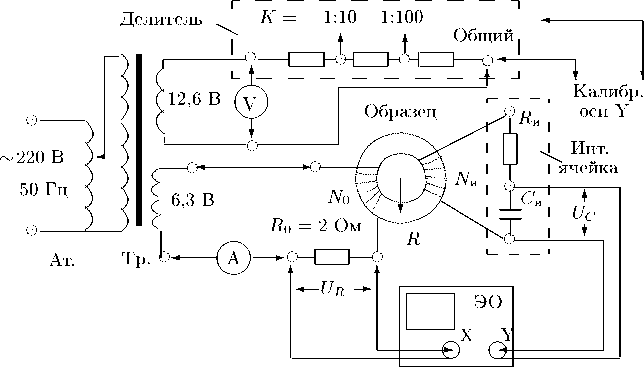
\includegraphics{./media/image8.png}

Рис. 2. Схема установки для исследования намагничивания образцов

Замкнутая кривая, возникающая на экране, воспроизводит в некото­ром
масштабе (различном для осей \emph{X и Y)} петлю гистерезиса. Чтобы
придать этой кривой количественный смысл, необходимо установить масштабы
изображения, т. е. провести калибровку каналов \emph{X} и \emph{Y} ЭО.
Для этого, во-первых, надо узнать, каким напряжениям (или токам)
соответствуют амплитуды сигналов, видимых на экране, и, во-вторых, каким
значениям \emph{В} и \emph{Н} соответствуют эти напряжения (или токи).

Напряжение, пропорциональное току в намагничивающей обмотке, подаётся на
горизонтальную ось Х. Если ручка усиления оси X в положении калибр, цену
деления по горизонтальной оси получим, разделив цену деления в вольтах
на сопротивление R\textsubscript{0} в амперах. Значения поля Н
рассчитыва­ются по теореме о циркуляции (см. (4.7){]}, Для
дополнительной проверки с помощью амперметра нужно закоротить обмотку
No, так как катушка с ферромагнитным образцом является нелинейным
элементом, ток в ней не име­ет синусоидальной формы, и связать амплитуду
тока с показаниями амперметра, измеряющим эффективное значение, можно
только с большой ошибкой..

При закороченной обмотке No показания эффективного тока, умноженные на
2√2, дадут удвоенное значение амплитуды тока, подаваемого на ось X,
соответствующего длине горизонтальной развёртки .Калибровка вертикальной
оси, как правило, не нужна.Но она может проводиться с помощью сигнала,
снимаемого через делитель напряжения с обмотки 12,6 В понижающего
трансформатора (рис. 2). Вольтметр V может достаточно точно измерить
напряжение U \textsubscript{эфф} , подаваемого на вход осциллографа.
После этого можно сравнить показания осциллографа и вольтметра.

Величина индукции B рассчитывается по формуле (4).

Постоянную времени RC'-цепочки можно определить экспери­ментально. С
обмотки 6,3 В на вход интегрирующей цепочки подаётся синусоидальное
напряжение Uвх. На вход Y осциллографа или цифрового вольтметра
поочерёдно подаются сигналы со входа (U \textsubscript{вх}) и выхода ( U
\textsubscript{вых}= Uc) RC-цепочки. Измерив амплитуды этих сигналов,
можно рассчитать постоянную времени τ = RC (формула (5)).

ЗАДАНИЕ

В работе предлагается при помощи ЭО исследовать предельные пет­ли
гистерезиса и начальные кривые намагничивания для нескольких
ферромагнитных образцов; определить магнитные характеристики
ма­териалов, чувствительность каналов X и Y осциллографа и постоянную
времени т интегрирующей цепочки.

Для наблюдения петли гистерезиса на экране ЭО соберите схему со­гласно
рис. 2. Подготовьте приборы к работе.

Подберите ток питания в намагничивающей обмотке и коэффициен­ты усиления
ЭО так, чтобы предельная петля гистерезиса занимала большую часть экрана
(при этом ширина петли при увеличении тока практически не меняется).

Зарисуйте на кальку предельную петлю и оси координат; отметьте на осях
деления шкалы. Укажите (на кальке!) материал образца, зна­чения
коэффициентов усиления Кх и Ку осциллографа, ток I \textsubscript{эфф} в
намагничивающей обмотке, параметры тороида.

Снимите начальную кривую намагничивания: плавно уменьшая ток
намагничивания до нуля, отмечайте на кальке вершины наблюдаемых частных
петель. Эти вершины лежат на начальной кривой намагничи­вания.

Восстановите предельную петлю. Измерьте на экране (это точнее, чем по
кальке) двойные амплитуды для коэрцитивной силы {[}2х(с){]} и индукции
насыщения {[}2y(s). Запишите соответствующие значения Кх и Ку.

Повторите измерения пп. 2-4 для двух других катушек.

Прокалибруйте горизонтальную ось ЭО. Для этого отключите
на­магничивающую обмотку No от цепи и снимите длину развёртки по оси X
при токе I\textsubscript{эфф}, близком к току насыщения петли
гистерезиса.

Для проверки калибровки вертикальной оси ЭО подключите вольтметр и
осциллограф к делителю 1:100(рис. 2)и сравните показания вольтметра и
осциллографа при развёртке а ветикали пчти на весь экран. Оцените
погрешность.

Определите τ--- постоянную времени RC-цепочки (см. (9){]}. Для этого
разберите цепь тороида и подайте на вход RC-цепочки синусоидальное
напряжение с обмотки 6,3 В трансформатора.

Измерьте отношение с помощью осциллографа и вольтметра. Рассчитайте на
месте постоянную времени т = RC по формуле (5) и сравните с расчётом
через параметры Д„ и Си, указанные на установке.

Запишите параметры RС-цепочки, амперметра, вольтметра и значе­ние RC.

\protect\hypertarget{bookmark66}{}{}Обработка результатов

Сравните экспериментальное значение τ с расчётом через парамет­ры
R\textsubscript{и} и Си, указанные на установке.

Рассчитайте напряжённости поля Н в тороиде, поставив в соответствие
деления по оси X величине поля в А/м.

Рассчитайте коэрцитивную силу Нс, используя измеренное значе­ние 2х(с).

Рассчитайте Bs по формуле (6), взяв значения R\textsubscript{и} и Си,
указанные на установке. Укажите на кальках масштабы для предельных
петель: Н {[}А/м{]} на одно деление; В{[}Т{]} на одно деление
рассчи­тайте по формуле (6), взяв вместо U\textsubscript{вых} .Оцените
начальные и максимальные значения µ\textsubscript{диф} по основным
кривым намаг­ничивания.

Оцените погрешности. Сведите результаты в таблицу:

\begin{longtable}[]{@{}llll@{}}
\toprule
Ампл. & Fe-Ni & Fe-Si & Феррит\tabularnewline
\midrule
\endhead
\begin{minipage}[t]{0.24\columnwidth}\raggedright\strut
Нс А Bs Тл

Мдиф\strut
\end{minipage} & \begin{minipage}[t]{0.24\columnwidth}\raggedright\strut
эксп.

табл.\strut
\end{minipage} & \begin{minipage}[t]{0.24\columnwidth}\raggedright\strut
\strut
\end{minipage} & \begin{minipage}[t]{0.24\columnwidth}\raggedright\strut
\strut
\end{minipage}\tabularnewline
\bottomrule
\end{longtable}

\protect\hypertarget{bookmark67}{}{}Контрольные вопросы

При какой форме образцов, помещённых в однородное магнитное поле, их
намагниченность постоянна по всему объёму?

Почему для наблюдения петли гистерезиса используются образцы в виде
тора, а не в виде стержня?

Почему при калибровке горизонтальной оси осциллографа необходимо
от­ключать намагничивающую обмотку?

4? Оцените погрешность, которая возникает при измерении индукции В, если
измерительная катушка неплотно надета на образец; например, если образец
занимает всего половину охватываемой ею площади.

СПИСОК ЛИТЕРАТУРЫ

Сивухин Д.В. Общий курс физики. Т. III. Электричество. --- М.: Наука,
1983. §§ 74, 79.

Калашников С.Г. Электричество. --- М.: Наука, 1977. §§ 110, 111, 119.

Кингсеп А.С., Локшин Г.Р., Ольхов О.А. Основы Физики. Т. 1. Механика,
электричество и магнетизм, колебания и волны, волновая оптика. --- М.:
Физ- матлит, 2001. Ч. II, гл. 5, § 5.3.

\end{document}
